%%%%%%%%%%%%%%%%%%%%%%%%%%%%%%%%%%%%%%%%%
% a0poster Landscape Poster
% LaTeX Template
% Version 1.0 (22/06/13)
%
% The a0poster class was created by:
% Gerlinde Kettl and Matthias Weiser (tex@kettl.de)
% 
% This template has been downloaded from:
% http://www.LaTeXTemplates.com
%
% License:
% CC BY-NC-SA 3.0 (http://creativecommons.org/licenses/by-nc-sa/3.0/)
%
%%%%%%%%%%%%%%%%%%%%%%%%%%%%%%%%%%%%%%%%%

%----------------------------------------------------------------------------------------
%	PACKAGES AND OTHER DOCUMENT CONFIGURATIONS
%----------------------------------------------------------------------------------------

\documentclass[a0,landscape]{a0poster}

\usepackage{multicol} % This is so we can have multiple columns of text side-by-side
\columnsep=100pt % This is the amount of white space between the columns in the poster
\columnseprule=3pt % This is the thickness of the black line between the columns in the poster

\usepackage[svgnames]{xcolor} % Specify colors by their 'svgnames', for a full list of all colors available see here: http://www.latextemplates.com/svgnames-colors

\usepackage{times} % Use the times font
%\usepackage{palatino} % Uncomment to use the Palatino font

\usepackage{graphicx} % Required for including images
\graphicspath{{../Analyse/out/}} % Location of the graphics files
\usepackage{booktabs} % Top and bottom rules for table
\usepackage[font=small,labelfont=bf]{caption} % Required for specifying captions to tables and figures
\usepackage{amsfonts, amsmath, amsthm, amssymb} % For math fonts, symbols and environments
\usepackage{wrapfig} % Allows wrapping text around tables and figures
\usepackage{natbib}


\renewcommand\bibsection{\subsubsection*{References}}

\begin{document}

%----------------------------------------------------------------------------------------
%	POSTER HEADER 
%----------------------------------------------------------------------------------------

% The header is divided into three boxes:
% The first is 55% wide and houses the title, subtitle, names and university/organization
% The second is 25% wide and houses contact information
% The third is 19% wide and houses a logo for your university/organization or a photo of you
% The widths of these boxes can be easily edited to accommodate your content as you see fit

\begin{minipage}[b]{0.55\linewidth}
\veryHuge \color{NavyBlue} \textbf{Don't Just Ask Me for Facts!} \color{Black}\\ % Title
\Huge\textit{Measuring Political Sophistication Using Open-Ended Responses}\\[1cm] % Subtitle
\huge \textbf{Patrick W. Kraft}\\ % Author(s)
\huge Stony Brook University, Department of Political Science\\ % University/organization
\end{minipage}
%
\begin{minipage}[b]{0.25\linewidth}
\color{DarkSlateGray}\Large \textbf{Contact Information:}\\
Department of Political Science\\ % Address
Social and Behavioral Sciences Building\\
Stony Brook University, Stony Brook, NY 11794\\\\
Phone: +1 (631) 371 1607\\ % Phone number
Email: \texttt{patrick.kraft@stonybrook.edu}\\ % Email address
\end{minipage}
%
\begin{minipage}[b]{0.19\linewidth}
\hspace{5cm}\includegraphics[width=12cm]{/data/Dropbox/Uni/Misc/Logos/SBU_vert1_2clr.jpg}\\\\
\end{minipage}

\vspace{1cm} % A bit of extra whitespace between the header and poster content

%----------------------------------------------------------------------------------------

\begin{multicols}{4} % This is how many columns your poster will be broken into, a poster with many figures may benefit from less columns whereas a text-heavy poster benefits from more

\color{Navy} % Navy color for the abstract
\begin{abstract}
There is a broad consensus among scholars of political science and public opinion that the American electorate is not well informed about politics. However, there is no agreement in the discipline about \textit{how to measure} how little citizens actually know. While many studies rely on simple factual political knowledge questions to assess political sophistication, others have criticized this approach from methodological and theoretical perspectives, claiming it does not provide a valid measure of the concept of interest. Using data from the 2012 American National Election Study (ANES), I propose an alternative measure of political sophistication based on open-ended survey responses about political preferences. The text-based metric captures aspects of sophistication unaccounted for when using conventional knowledge indices and is conceptually closer to theoretical approaches that emphasize the importance of the structure and complexity of belief systems.
\end{abstract}

\color{SaddleBrown} % SaddleBrown color for the introduction
%\color{Black}
\section*{Issues with Political Knowledge}
\begin{itemize}
   \item Biases due to guessing \citep[e.g.][]{mondak2004knowledge}
   \item Partial knowledge \citep[e.g.][]{debell2013harder}.
   \item Conditional on motivation \citep[e.g.][]{prior2008money}
   \item Ignores important aspects such as visual cues \citep{prior2014visual}
   \item Convolutes different types of knowledge \citep{barabas2014question}
   \item Not relevant for participation \citep{lupia2006elitism}
   \item Does not capture belief system constraint \citep{luskin1987measuring,tetlock1983cognitive}
\end{itemize}

%\color{DarkSlateGray} % DarkSlateGray color for the rest of the content
\color{Black} % DarkSlateGray color for the rest of the content
\section*{Description of Alternative Measure}

The measure is based on open-ended responses where individuals list anything that they like/dislike about the Democratic/Republican party as well as anything that might make them vote/not vote for either of the Presidential candidates. The analyses presented here are based on the 2012 ANES (2054 f2f, 3860 online respondents). Verbatim responses were pre-processed using an implementation of the Aspell spell checking algorithm in R, and eliminating non-English responses (228 individuals). 
\vspace{1em}

\begin{center}
\begin{tabular}{p{15cm}p{10cm}}
\toprule 
Political belief system & Open-ended response \\
\midrule
Size (number of cognitions) & Overall length of responses \\
Range (dispersion over categories) & Topic diversity \\
Constraint (interconnectedness) & Response diversity \\
\bottomrule
\end{tabular}
\captionof{figure}{\color{Green} Dimensions of political belief system as aspects of political sophistication and their measure in open-ended responses \citep[c.f.][]{luskin1987measuring}.}
\end{center}

\begin{align}
\text{size}_i &= \dfrac{\log\left(\sum_{j=1}^J n_{ij}\right)}{\max\left[\log\left(\sum_{j=1}^J n_{ij}\right)\right]},\\
\text{range}_i &= 1-\dfrac{\sum_{k_1=1}^K\sum_{k_2=1}^K |\theta_{ik_1} - \theta_{ik_2}|}{2\sum_{k_1=1}^K\sum_{k_2=1}^K \theta_{ik_1}},\\
\text{constraint}_i &= 1-\dfrac{\sum_{j_1=1}^J\sum_{j_2=1}^J |p_{ij_1} - p_{ij_2}|}{2\sum_{j_1=1}^J\sum_{j_2=1}^J p_{ij_1}},\\
\text{sophistication}_i &= \text{size}_i * \text{range}_i * \text{constraint}_i.
\end{align}

\begin{center}
\begin{tabular}{lp{22cm}}
\toprule 
$i$ & Individual respondent \\
$j \in J$ & Like/dislike items (8 total) \\
$k \in K$ & Topics (72 total, estimated via STM using spectral initialization, c.f. \citealt{roberts2014structural}) \\
$\theta_{ik}$ & predicted proportion of topic $k$ in the collection of responses by individual $i$\\
$p_{jk}$ & proportion of words in the response of individual $i$ to question $j$ relative to the overall size of the individual's response\\
\bottomrule
\end{tabular}
\end{center}

\begin{center}\footnotesize
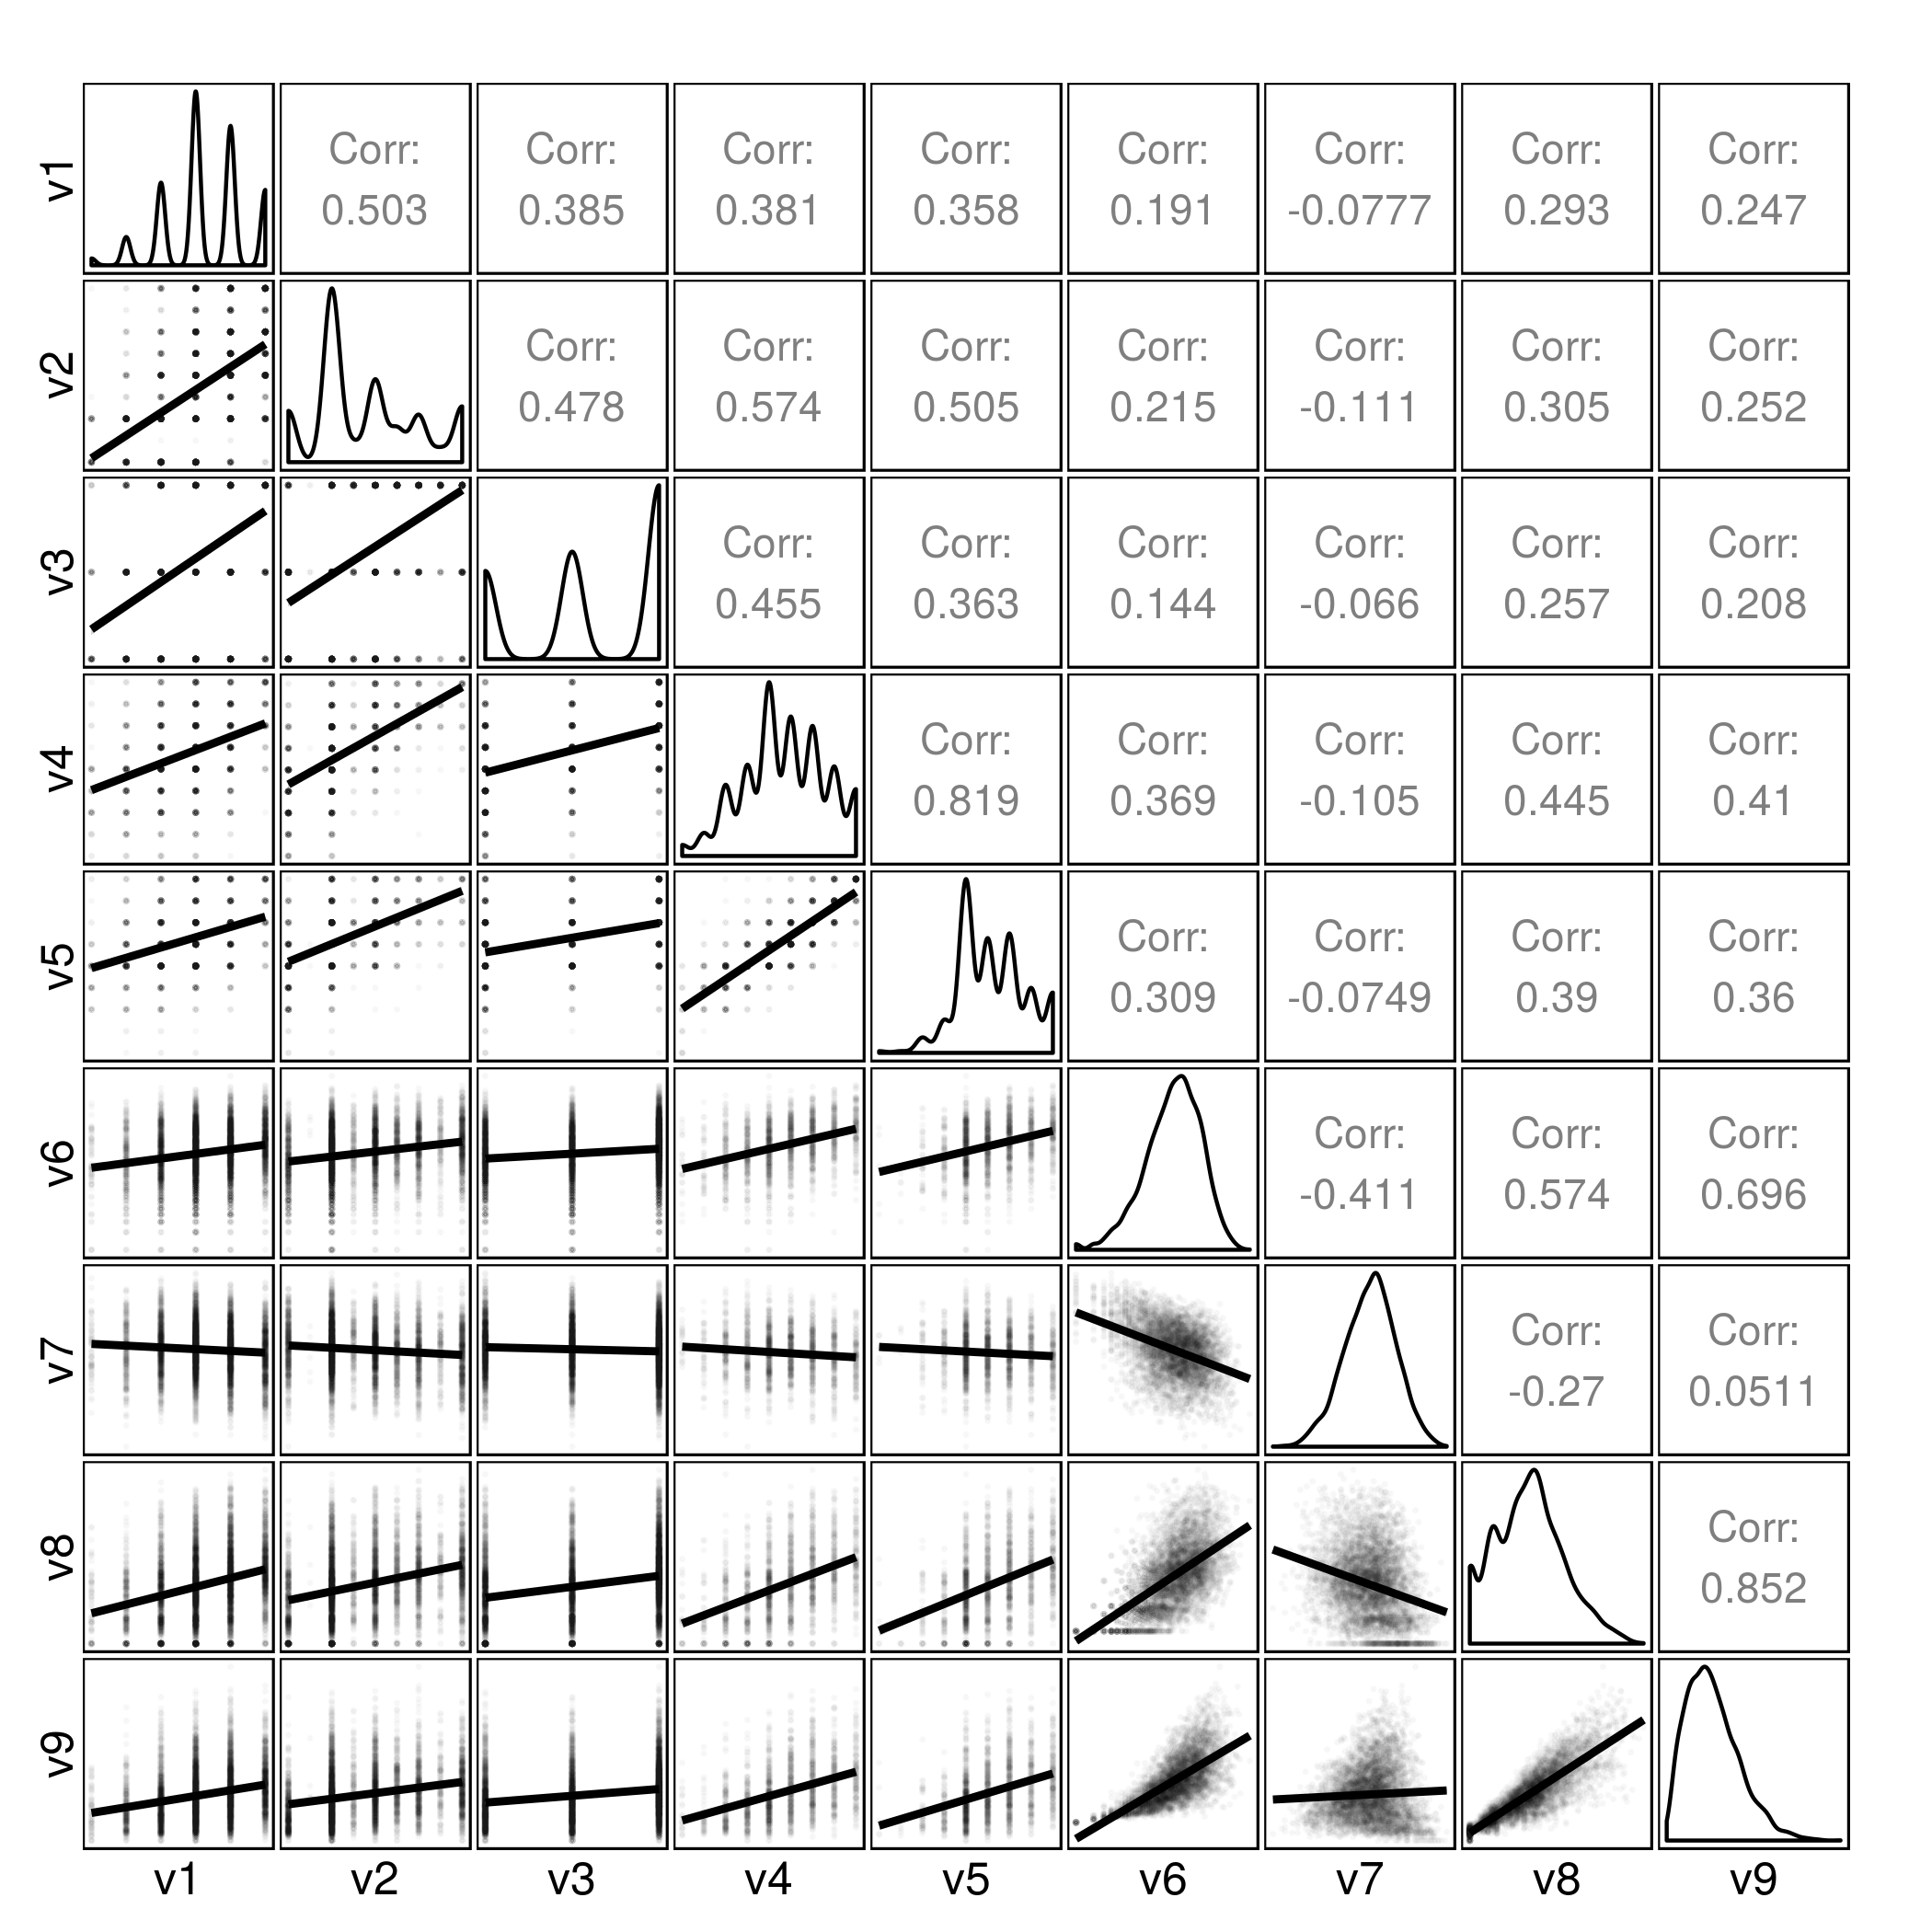
\includegraphics[width=\linewidth]{figures/corplot.png}
\begin{tabular}[ht]{llllll}
\toprule
v1 & Factual Knowledge & v4 & Political Knowledge (Int. Eval.) & v7 & Topic Diversity \\
v2 & Office Recognition & v5 & Intelligence (Int. Eval.) & v8 & Response Diversity \\
v3 & Majorities in Congress & v6 & Total Response Length &  v9 & Text-based Sophistication \\
\bottomrule
\end{tabular}
\captionof{figure}{\color{Green} Correlation matrix of conventional political knowledge metrics, the text-based sophistication measure, as well as its individual components. The figures on the diagonal display unvariate densities for each variable.}
\end{center}

The text-based sophistication measure is positively correlated with all conventional metrics while capturing some additional variation. However, one of the components of the text-based measure, Topic Diversity (v7), shows low negative correlations with all other indices. One explanation for this finding is that the posterior topic proportions of the structural topic model are strongly affected by the prior over topics for short responses. The text-based sopistication measure is positively correlated with the interviewer's assessment of the respondent's apparent intelligence, although less so than other conventional metrics as well as less than with the interviewer's assessment of the respondent's level of information.

\begin{center}\footnotesize
\begin{tabular}[ht]{lp{10.5cm}p{10.5cm}}
   \toprule
  & Low & High \\ 
   \midrule
   Obama (+) &  & i think he has done well so far \\ 
   Obama (-) & Shady. He left his spot in Illinois and someone is in prison for trying to sell it. Wonder how he got it. Probably the same way he got the Nobel. Who's in charger of USDA school program? Who is surgeon General? How they get there? What are their true credentials prior to current positions? Reeks. & way things are going with education \\ 
   Romney (+) &  & his health policy outlooks, but it also hinders itself as well. his pro-life opinion \\ 
   Romney (-) &  & personality a lot of his policies \\ 
   Democrats (+) &  & i like their ideas they are for the people \\ 
   Democrats (-) & They care about the stupidest stuff & sometimes i wonder if progress can occur \\ 
   Republicans (+) &  & my religous beliefs of Christianity tend to follow many of their thoughts \\ 
   Republicans (-) & Stewards for the rich and big business & soemtimes they don't make sense or have just never been 'the right mix' to make me want to vote for them \\ 
    \bottomrule
    \end{tabular}
  \captionof{table}{\color{Green} Example of open-ended responses for low and high scores of text-based sophistication measure with equal response length (between 50 and 100 words). Note that these are the raw responses without any pre-processing (spell-checking etc.).}
  \end{center}


\section*{Validation I: Determinants of Sophistication}
\begin{center}
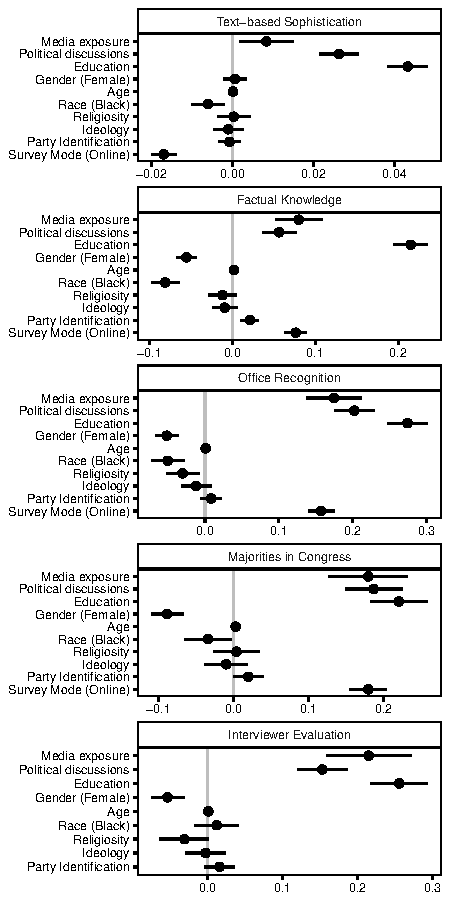
\includegraphics[width=\linewidth]{figures/models.pdf}
\captionof{figure}{\color{Green} Common determinants of political sophistication and political knowledge. Estimates are OLS regression coefficients with 95\% confidence intervals. Dependent variables are the text-based sophistication measure as well as conventional metrics.}
\end{center}

Figure 3 compares the effects of common determinants of political sophistication and knowledge for the different measures. While the overall patterns are consistent across metrics, there are some interesting differences regarding the text-based measure. The gender-bias frequently reported using traditional indicators of political knowledge disappears when sophistication is measured using open-ended responses. Women might not score as high on political information quizzes (partly because they are less likely to guess rather than to express lack of knowledge, c.f. \citealt{mondak2004knowledge}), but they do not differ substantially in complexity and sophistication when they describe their political preferences. Furthermore, the effect of survey mode is reversed, which can be explained by the fact that factual questions in online surveys can overestimate knowledge when respondents look up ansewers \citep[see also][]{clifford2016cheating}.

\section*{Validation II: Coherent Attitudes}
\begin{center}
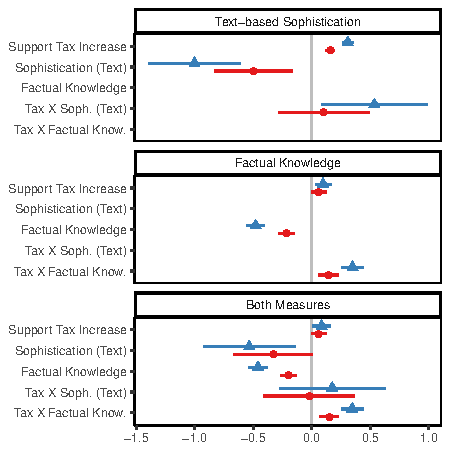
\includegraphics[width=\linewidth]{../fig/models2.pdf}
\captionof{figure}{\color{Green} Sophistication and Coherent Attitudes. Estimates are OLS regression coefficients with 95\% confidence intervals. The dependent variable measures support for redistributive economic policies. Red circles indicate model results including control variables such as gender, age, race, religiosity, ideology, and party identification.}
\end{center}

Similar to the analyses in \citet{prior2014visual}, Figure 4 examines whether sophistication increases the consistency between related political preferences (i.e. coherence between support for tax increase for high incomes and support for redistributive policies). Positive interaction effects indicate that sophistication increases coherence. The results suggest that factual political knowledge is a better predictor of consistent preferences.


%\color{SaddleBrown} % SaddleBrown color for the introduction
%\section*{Conclusion}

\vspace{2em}

%----------------------------------------------------------------------------------------
%	REFERENCES
%----------------------------------------------------------------------------------------


\color{Black} % SaddleBrown color for the introduction
\begin{tiny}
\setlength{\parskip}{-5pt}
\bibliographystyle{/data/Dropbox/Uni/Lit/apsr2006}
\bibliography{/data/Dropbox/Uni/Lit/Literature}
\end{tiny}

%----------------------------------------------------------------------------------------
%	ACKNOWLEDGEMENTS
%----------------------------------------------------------------------------------------

\subsubsection*{Acknowledgements}
\setlength{\parskip}{-20pt}
%\begin{footnotesize} 
I thank Laura Buchanan for her work on previous versions of this paper as well as Jennifer Jerit, Yanna Krupnikov, and Stanley Feldman for helpful comments.
%\end{footnotesize} 

%----------------------------------------------------------------------------------------

\end{multicols}
\end{document}